\section{Other Android Security Challenges}
One of the principal reasons that the Android platform suffers from a plethora of security issues is fragmentation \cite{Zhou2014, Gilski2015, Faruki2015}.
The fragmentation of the Android platform is derived from the various customizations new devices undergo during development.
Customizations may include hardware drivers and pre-installed applications.
As stated prior, the hardware drivers that exist in the Android platform are a significant source of vulnerabilities.

Since the implications and mechanics of the vulnerabilities at the low-level parts of the stack have been discussed at length in Section II, the main focus of this section will be on the applications.
A study done by Zhou \etal discusses the security implications of Android's fragmentation issue \cite{Zhou2014}.
In the study, the researchers found that the topic was not well researched and that different images of the Android OS customized by hardware vendors contained security vulnerabilities.
Particularly, a number of apps that came pre-installed on some images were given excessive privileges, among other issues.

In regard to responsible application development, Android applications are not always up to an acceptable standard.
Web applications are a large source of vulnerabilities, which opens them up to network-based attacks.
Third party libraries (code libraries written to assist in application development with the goal of reducing the burden of implementing complicated or repetitive aspects of other programs) are also a common source of vulnerabilities.
The reason for these vulnerabilities seems to be, in large part, by developers who are either unaware of the potential vulnerabilities of their system, a lack of awareness or domain knowledge of the components used in their system, or a lack of understanding for how to use a particular technology \cite{Qin2020, Zhan2021}.

One domain of misuse includes OAuth implementations. OAuth is an open standard for access control mechanisms built into Internet services.
A common use case is to use the standard in an application to access the information of a service from another service or application if user permission is given.
A study conducted by Wang \etal found that applications vendored by both American (specifically the Google Play Store) and Chinese Android app markets demonstrated misuse of the OAuth protocol \cite{Wang2015}.
Part of the reason for this seemed to be a lack of understanding of the specifications by the developers.
Figure \ref{fig:OAuth2Oracle}, sourced from Oracle's documentation \cite{OAuth2ControlOracle}, demonstrates a typical control flow for the OAuth 2.0 protocol.

\begin{figure}[htbp]
    \centerline{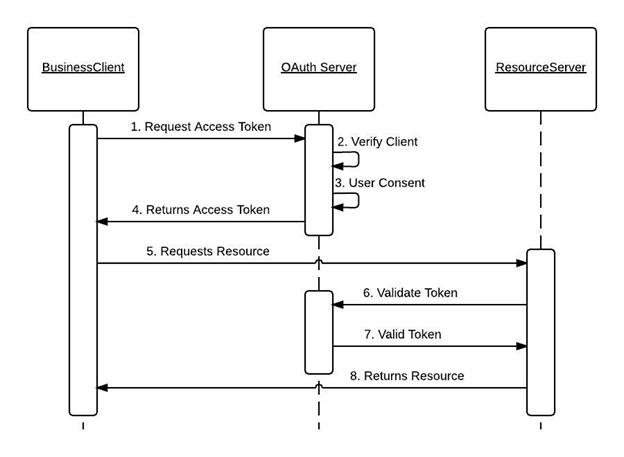
\includegraphics[width=0.5\textwidth]{figures/OAuth2Oracle.png}}
    \caption{OAuth 2.0 protocol control flow.}
    \label{fig:OAuth2Oracle}
\end{figure}

Another misuse case may be derived from a native library supported by the Android platform: SQLite \cite{SQLite}.
SQLite is a widely used embeddable SQL relational database engine.
SQLite, like other SQL databases, is susceptible to query injection \cite{Maalouf2021}.

Expanding on SQLite some more, a peculiar quirk that sets it apart from other SQL databases is access control.
SQLite effectively have no access control mechanisms because the file is stored on disk (access to that file may be controlled like any other, but it does not extend to the tables, columns, rows, etc. stored in the file).
Mutti \etal propose an SELinux-like model to the SQLite database included in the Android platform to improve access control to databases stored on-device \cite{Mutti2015}.
Since applications on Android are sandboxed and are assigned their own user identifier, permissions could be given to certain applications to access only the subset of the database it needs, allowing applications to exchange data securely.

Application development on the Android platform could be significantly improved with the invention of tools that assist in the testing and verification of code safety.
Developers could find themselves under significant time pressure, might be using unfamiliar components or standards, or may engage in happy-path testing.
Programmers could produce poor quality code for any number of reasons.
Tools and automation are consistent when developing sensitive systems and may help reduce the human aspect of flawed software.
